\section{Introduction}
This paper seeks to discuss different methods to automate the measurement of cartilage thickness in the human knee using MRI scans. The methods are based on previous work by Wolfgang Wirth and Felix Eckstein. \cite{wirth2008technique}
\par\noindent
All computational methods make use of segmented MRI scans of the human knee, from the OAI dataset, and are written in Python. The segmentations are stored as MHD files, which can be read and converted into Numpy arrays using the SimpleITK library. These arrays map each point in the three-dimensional space of the scan to an integer encoding, meaning for example points belonging to the femoral cartilage are assigned a value of 3. This makes isolating and extracting the cartilage volumes straightforward. Four different methods have been developed to determine mean cartilage thickness, plus other statistical measures.

\section{Mean cartilage thickness using meshes}
This is a three-dimensional approach using meshes and normal vectors to determine the mean thickness of a cartilage volume. The main idea is building an upper and a lower mesh, and calculating the average distance between the two, for example by ray tracing along the normal vectors of the lower mesh against the upper mesh. Other methods, like a K-D-tree nearest neighbour search, are also possible. This works well for the tibial cartilage, because due to its physical shape, it is possible to simply group each point by $x$ and $y$ coordinates and add the point with the highest (lowest) $z$ coordinate to the upper (lower) mesh. The result is two point clouds consisting of vectors $(x, y, z)$, as seen in figure \ref{fig:tibial_point_cloud} (red points make up the upper cloud, green the lower). These can then be converted into polygon meshes using the delaunay algorithm, which in turn allows for determining the normal vectors of the respective meshes. Mean cartilage thickness can be calculated by tracing along the normal vectors of the lower mesh against the upper mesh. For other methods not making use of the normals, like the previously mentioned nearest neighbour search, the delaunay conversion is optional. 
\begin{figure}[htb!]
	\centering
	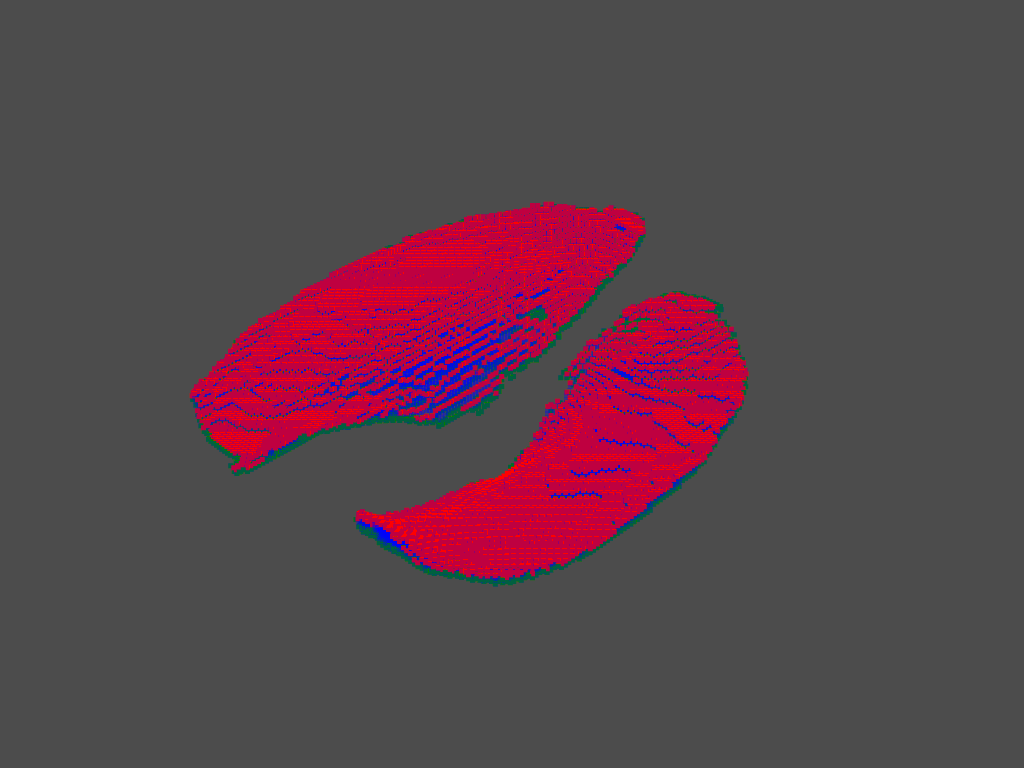
\includegraphics[width=\linewidth]{./figures/s2}
	\caption{Point clouds of the tibial cartilage}
	\label{fig:tibial_point_cloud}
\end{figure}
\par
The femoral cartilage makes things a bit more tricky. Due to its shape, building an upper and lower mesh is not trivial, because while for the tibial cartilage, there was only one respective vector for each coordinate pair $(x, y)$, there may now be multiple for the areas where the volume describes a curve, so just taking the minimum or maximum $z$ coordinate no longer suffices. Using the previous approach results in point clouds where some areas are left bare, as illustrated in figure \ref{fig:femoral_point_cloud}. One solution, used in this approach, is splitting the volume into parts, and rotating the curved sections, such that it is once again possible to choose points according to the $z$ coordinate. This allows for building an upper and lower point cloud and corresponding delaunay mesh for each part, calculating the mean distance in the same manner as before (aka ray tracing), and finally combining the results.
\begin{figure}[htb!]
	\centering
	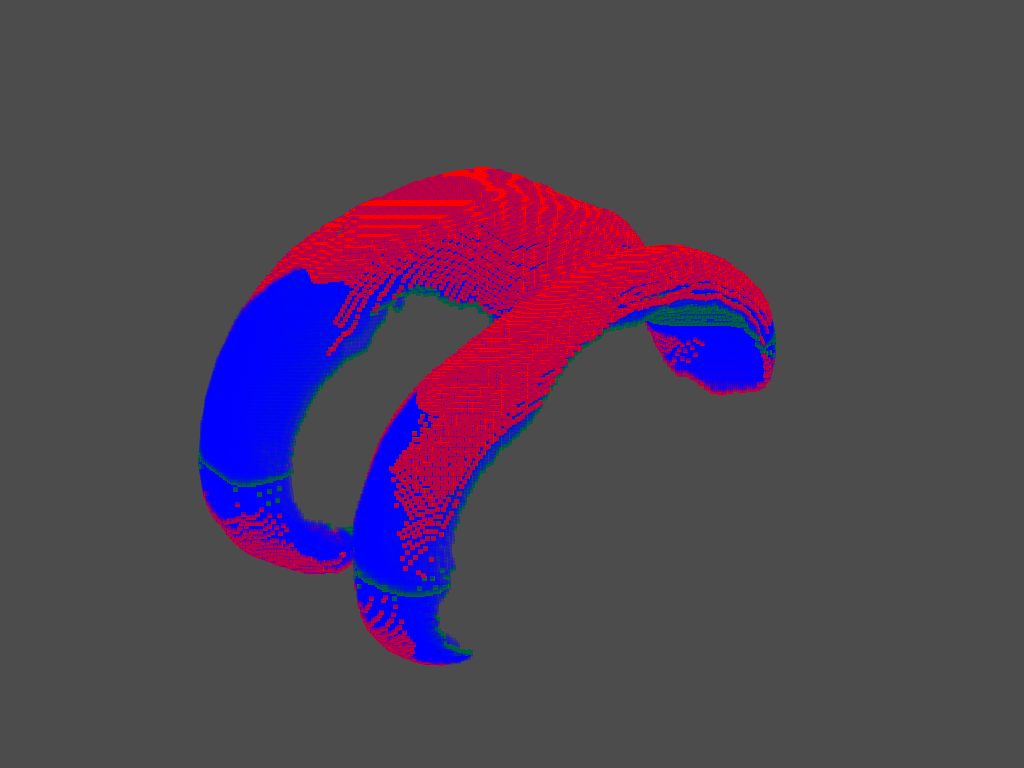
\includegraphics[width=\linewidth]{./figures/s4}
	\caption{Point clouds of the femoral cartilage}
	\label{fig:femoral_point_cloud}
\end{figure}

\section{Mean cartilage thickness using ray tracing from a central point}
This is a three-dimensional approach using ray tracing along normal vectors to determine the mean thickness of a cartilage volume. This is another proposed solution to the previously discussed issue with the shape of the femoral cartilage volume. Instead of using meshes, this approach takes a central point underneath or above the cartilage and utilizes ray tracing from that point against the volume to discover intersection points. 
\par
A sphere is constructed around the central point, and each of its normal vectors gets extended until it hits the cartilage point cloud, or a maximum number of iterations is reached. If a point is hit, it is saved and the vector again gets extended until it doesn't hit any points anymore, i.e. it is extended past beyond the cartilage. The distance between the first and last point hit is calculated and added to the result set. This way, it is possible to determine the average thickness of the cartilage. One issue with this approach is that it is computationally expensive, as intersection problems tend to be; in essence, there is a trade-off between accuracy and runtime: The more vectors are used for the ray tracing, the more accurate the result is going to be, but each added vector makes the computation more expensive.
\begin{figure}[htb!]
	\centering
	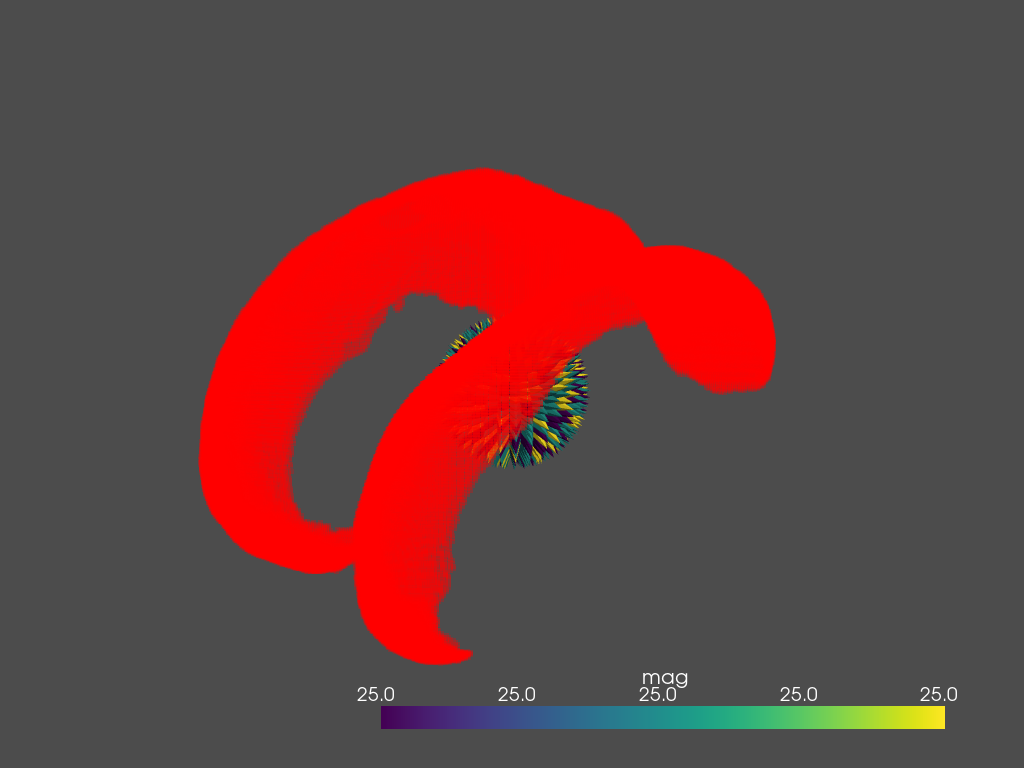
\includegraphics[width=\linewidth]{./figures/s5}
	\caption{Ray tracing against the femoral cartilage using a central sphere}
	\label{fig:femoral_sphere}
\end{figure}

\section{Mean cartilage thickness using two-dimensional function fitting}
\subsection{Determine thickness via function normals}
This is a two-dimensional approach using a least-squares fit of single cartilage layers to determine the mean thickness of a cartilage volume. As the MRI scans consist of a number of slice exposures, it is possible to do the thickness calculation layer by layer. For each layer, a polynomial function gets fitted over the data points, i.e. through the middle of the volume, and a variable number of normals is calculated along the fitted function. For each normal, the inner- and outermost intersection points with the cartilage are determined, and the distance between these to points is added to the result set, as illustrated in figure \ref{fig:normals}.
\begin{figure}[htb!]
	\centering
	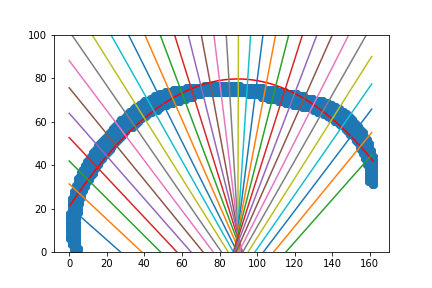
\includegraphics[width=\linewidth]{./figures/normals}
	\caption{Normals along a two-dimensional least squares fit}
	\label{fig:normals}
\end{figure} 

\subsection{Determine thickness via integration/function values}
This is another two-dimensional variant, where two functions are fitted over the data points, i.e. not through the middle of the volume but rather along the outlines of the volume, as illustrated in figure \ref{fig:integration}. The distance between the functions, i.e. the thickness of the cartilage, can then easily be calculated, for example by integrating both functions and taking the difference ($\int f(x) dx - \int g(x) dx$), or calculating the difference between the function values for every $x$ value ($[\sum_{x_i = 0}^{max(x)} f(x_i) - g(x_i)] \cdot \frac{1}{max(x)}$).
\par
One issue with both of these approaches is that the function fitting may not work well for certain shapes, especially for layers where the number of data points is very sparse.
\begin{figure}[htb!]
	\centering
	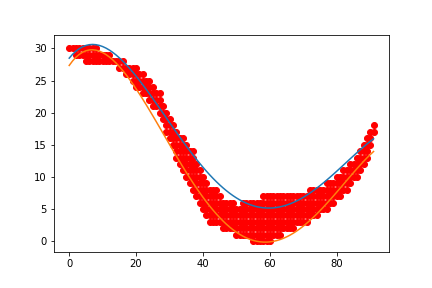
\includegraphics[width=\linewidth]{./figures/integration}
	\caption{Two functions fit over the outlines of a tibial cartilage slice exposure}
	\label{fig:integration}
\end{figure}